
%(BEGIN_QUESTION)
% Copyright 2009, Tony R. Kuphaldt, released under the Creative Commons Attribution License (v 1.0)
% This means you may do almost anything with this work of mine, so long as you give me proper credit

Calculating gas flow rates through a control valve is a bit more complex than calculating liquid flow rates.  One standard equation for gas flow through a valve, assuming the absence of choking (sonic, or {\it critical}, gas velocity in the valve), is as follows:

$$Q = 963 \> C_v \sqrt{{\Delta P (P_1 + P_2)} \over {G_g T}}$$

\noindent
Where,

$Q$ = Gas flow rate, in units of Standard Cubic Feet per Hour (SCFH)

$C_v$ = Valve capacity coefficient

$\Delta P$ = Pressure dropped across valve, pounds per square inch differential (PSID)

$P_1$ = Upstream valve pressure, pounds per square inch absolute (PSIA)

$P_2$ = Downstream valve pressure, pounds per square inch absolute (PSIA)

$G_g$ = Specific gravity of gas (Air at standard temperature and pressure = 1.0)

$T$ = Absolute temperature of gas in degrees Rankine ($^{o}$R)

\vskip 10pt

Using this ``subcritical'' formula for gas flow through a valve, determine the amount of air flow through this valve when it is wide open:

$$\includegraphics[width=15.5cm]{i01412x01.eps}$$

Assume room temperature (70$^{o}$ F) for the air flowing through the valve.

\vskip 10pt

Also, explain why it would be important to specify the proper {\it ANSI flange class} when ordering a control valve for this application.

\vskip 20pt \vbox{\hrule \hbox{\strut \vrule{} {\bf Suggestions for Socratic discussion} \vrule} \hrule}

\begin{itemize}
\item{} Explain why, when selecting the proper ANSI class for pipe flanges and valves, {\it temperature} is just as important a variable to consider as static {\it pressure}.
\end{itemize}

\underbar{file i01412}
%(END_QUESTION)





%(BEGIN_ANSWER)

$Q$ = 7,689.91 SCFH
 
%(END_ANSWER)





%(BEGIN_NOTES)

$$Q = 963 \> C_v \sqrt{{\Delta P (P_1 + P_2)} \over {G_g T}}$$

$$Q = (963) (0.5) \sqrt{{(1000 - 930) (1000 + 930)} \over {(1) (70 +459.67)}} = 7689.91 \hbox{ SCFH}$$

\vskip 10pt

This gas flow equation was derived from one found on page 27 of Hans D. Baumann's book, {\it Control Valve Primer, a user's guide}, second edition.  Other gas flow equations exist, and are generally more complex than this, accommodating piping geometry and other factors into the calculation.

\vskip 10pt

Given the high working pressure of this control valve, the pipe and pipe flanges must be suitably rated for safe and reliable operation.  It is critical that the valve's pressure-class match that of the mating flanges on the pipes.

%INDEX% Final Control Elements, valve: sizing

%(END_NOTES)


